\documentclass[tikz,border=10pt]{standalone}
\usepackage{tikz}
\usetikzlibrary{calc}
\usepackage[utf8]{inputenc}
\usepackage{sansmath}
\sansmath
\renewcommand{\familydefault}{\sfdefault}

\begin{document}
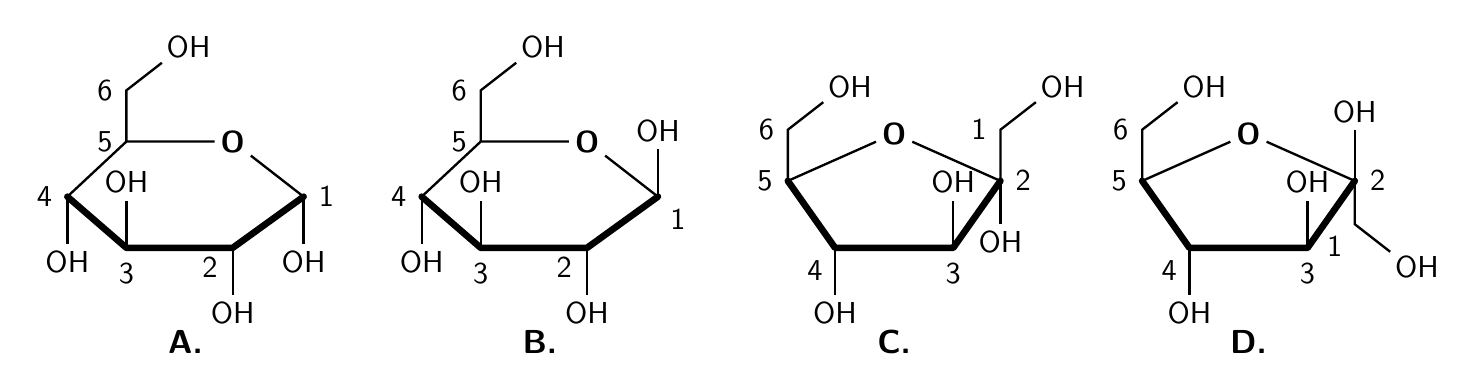
\begin{tikzpicture}[x=1cm, y=1cm, >=stealth, font=\sffamily\fontsize{10.5pt}{13pt}\selectfont]

% ==================== MOLECULE A ====================
\begin{scope}[shift={(0,0)}]
  % Ring vertices
  \coordinate (C4) at (-1.5, 0);
  \coordinate (C5) at (-0.75, 0.7);
  \coordinate (C1) at (1.5, 0);
  \coordinate (C2) at (0.6, -0.65);
  \coordinate (C3) at (-0.75, -0.65);

  % Ring Oxygen as a node on the vertex
  \node[inner sep=2pt] (O) at (0.6, 0.7) {\textbf{O}};

  % Back bonds (thin)
  \draw[line width=0.85pt] (C4) -- (C5) -- (O) -- (C1);

  % Front bonds (thick Haworth perspective)
  \draw[line width=2.4pt, line cap=round, line join=round] (C4) -- (C3) -- (C2) -- (C1);

  % Substituents
  % C5 -> C6 -> OH
  \draw[line width=0.85pt] (C5) -- ++(0, 0.65) coordinate (C6) -- ++(0.45, 0.35) node[above right=-2pt] {OH};
  \node[left=1.5pt] at (C6) {6};
  \node[left=1.5pt] at (C5) {5};

  % C4 -> OH (down)
  \draw[line width=0.85pt] (C4) -- ++(0, -0.6) node[below=-1pt] {OH};
  \node[left=2pt] at (C4) {4};

  % C3 -> OH (up)
  \draw[line width=0.85pt] (C3) -- ++(0, 0.6) node[above=-1pt] {OH};
  \node[below=2pt] at (C3) {3};

  % C2 -> OH (down)
  \draw[line width=0.85pt] (C2) -- ++(0, -0.6) node[below=-1pt] {OH};
  \node[left=2pt] at ($(C2)+(0,-0.25)$) {2};

  % C1 -> OH (down) (alpha-D-glucopyranose)
  \draw[line width=0.85pt] (C1) -- ++(0, -0.6) node[below=-1pt] {OH};
  \node[right=2pt] at (C1) {1};

  % Option label
  \node at (0, -1.85) {\large\textbf{A.}};
\end{scope}

% ==================== MOLECULE B ====================
\begin{scope}[shift={(4.5,0)}]
  % Ring vertices
  \coordinate (C4) at (-1.5, 0);
  \coordinate (C5) at (-0.75, 0.7);
  \coordinate (C1) at (1.5, 0);
  \coordinate (C2) at (0.6, -0.65);
  \coordinate (C3) at (-0.75, -0.65);

  % Ring Oxygen as a node on the vertex
  \node[inner sep=2pt] (O) at (0.6, 0.7) {\textbf{O}};

  % Back bonds (thin)
  \draw[line width=0.85pt] (C4) -- (C5) -- (O) -- (C1);

  % Front bonds (thick Haworth perspective)
  \draw[line width=2.4pt, line cap=round, line join=round] (C4) -- (C3) -- (C2) -- (C1);

  % Substituents
  % C5 -> C6 -> OH
  \draw[line width=0.85pt] (C5) -- ++(0, 0.65) coordinate (C6) -- ++(0.45, 0.35) node[above right=-2pt] {OH};
  \node[left=1.5pt] at (C6) {6};
  \node[left=1.5pt] at (C5) {5};

  % C4 -> OH (down)
  \draw[line width=0.85pt] (C4) -- ++(0, -0.6) node[below=-1pt] {OH};
  \node[left=2pt] at (C4) {4};

  % C3 -> OH (up)
  \draw[line width=0.85pt] (C3) -- ++(0, 0.6) node[above=-1pt] {OH};
  \node[below=2pt] at (C3) {3};

  % C2 -> OH (down)
  \draw[line width=0.85pt] (C2) -- ++(0, -0.6) node[below=-1pt] {OH};
  \node[left=2pt] at ($(C2)+(0,-0.25)$) {2};

  % C1 -> OH (up) (beta-D-glucopyranose)
  \draw[line width=0.85pt] (C1) -- ++(0, 0.6) node[above=-1pt] {OH};
  \node[below right=1pt] at (C1) {1};

  % Option label
  \node at (0, -1.85) {\large\textbf{B.}};
\end{scope}

% ==================== MOLECULE C ====================
\begin{scope}[shift={(9.0,0)}]
  % Furanose ring vertices
  \coordinate (C5) at (-1.35, 0.2);
  \coordinate (C2) at (1.35, 0.2);
  \coordinate (C3) at (0.75, -0.65);
  \coordinate (C4) at (-0.75, -0.65);

  % Top Ring Oxygen node
  \node[inner sep=2pt] (O) at (0, 0.8) {\textbf{O}};

  % Back bonds (thin)
  \draw[line width=0.85pt] (C5) -- (O) -- (C2);

  % Front bonds (thick Haworth perspective)
  \draw[line width=2.4pt, line cap=round, line join=round] (C5) -- (C4) -- (C3) -- (C2);

  % Substituents
  % C5 -> C6 -> OH
  \draw[line width=0.85pt] (C5) -- ++(0, 0.65) coordinate (C6) -- ++(0.45, 0.35) node[above right=-2pt] {OH};
  \node[left=1.5pt] at (C6) {6};
  \node[left=2pt] at (C5) {5};

  % C4 -> OH (down)
  \draw[line width=0.85pt] (C4) -- ++(0, -0.6) node[below=-1pt] {OH};
  \node[below left=1pt] at (C4) {4};

  % C3 -> OH (up)
  \draw[line width=0.85pt] (C3) -- ++(0, 0.6) node[above=-1pt] {OH};
  \node[below=2pt] at (C3) {3};

  % C2 -> C1 -> OH (up) & C2 -> OH (down) (alpha-D-fructofuranose)
  \draw[line width=0.85pt] (C2) -- ++(0, 0.65) coordinate (C1) -- ++(0.45, 0.35) node[above right=-2pt] {OH};
  \node[left=1.5pt] at (C1) {1};
  \draw[line width=0.85pt] (C2) -- ++(0, -0.55) node[below=-1pt] {OH};
  \node[right=2pt] at (C2) {2};

  % Option label
  \node at (0, -1.85) {\large\textbf{C.}};
\end{scope}

% ==================== MOLECULE D ====================
\begin{scope}[shift={(13.5,0)}]
  % Furanose ring vertices
  \coordinate (C5) at (-1.35, 0.2);
  \coordinate (C2) at (1.35, 0.2);
  \coordinate (C3) at (0.75, -0.65);
  \coordinate (C4) at (-0.75, -0.65);

  % Top Ring Oxygen node
  \node[inner sep=2pt] (O) at (0, 0.8) {\textbf{O}};

  % Back bonds (thin)
  \draw[line width=0.85pt] (C5) -- (O) -- (C2);

  % Front bonds (thick Haworth perspective)
  \draw[line width=2.4pt, line cap=round, line join=round] (C5) -- (C4) -- (C3) -- (C2);

  % Substituents
  % C5 -> C6 -> OH
  \draw[line width=0.85pt] (C5) -- ++(0, 0.65) coordinate (C6) -- ++(0.45, 0.35) node[above right=-2pt] {OH};
  \node[left=1.5pt] at (C6) {6};
  \node[left=2pt] at (C5) {5};

  % C4 -> OH (down)
  \draw[line width=0.85pt] (C4) -- ++(0, -0.6) node[below=-1pt] {OH};
  \node[below left=1pt] at (C4) {4};

  % C3 -> OH (up)
  \draw[line width=0.85pt] (C3) -- ++(0, 0.6) node[above=-1pt] {OH};
  \node[below=2pt] at (C3) {3};

  % C2 -> OH (up) & C2 -> C1 -> OH (down) (beta-D-fructofuranose)
  \draw[line width=0.85pt] (C2) -- ++(0, 0.65) node[above=-1pt] {OH};
  \draw[line width=0.85pt] (C2) -- ++(0, -0.55) coordinate (C1) -- ++(0.45, -0.35) node[below right=-2pt] {OH};
  \node[below left=1pt] at (C1) {1};
  \node[right=2pt] at (C2) {2};

  % Option label
  \node at (0, -1.85) {\large\textbf{D.}};
\end{scope}

\end{tikzpicture}
\end{document}
